\documentclass{article}
\usepackage[brazil]{babel}
\usepackage[utf8]{inputenc}
\usepackage{graphicx}
\usepackage{float}
\usepackage{indentfirst}

\floatstyle{boxed}
\newfloat{codigo}{thp}{lop}
\floatname{codigo}{Código}

\title{
\includegraphics[scale=0.4]{logo}\\
Papagaio: o kernel}
\author{Rafael Cunha de Almeida\\ $<$almeidaraf@gmail.com$>$}

\begin{document}
\maketitle

\section{Setup}
A arquitetura intel precisa de vários passos de inicialização antes de chegar a
um ponto onde o kernel pode assumir o controle. Eu poderia fazer toda a
inicialização eu mesmo ou eu posso também usar um bootloader, como o grub.

O grub carrega meu kernel de uma partição EXT2, lê o formato ELF do executável
que eu gerei, carrega o kernel nas posições de memória
especificadas~\footnote{Na figura~\ref{fig:memoria} podemos ver como a memória
do computador é disposta. Vendo o desenho nesse endereço fica claro o porque
carregar o kernel a partir do endereço físico 0x100000} (veja o arquivo
papagaio.ld), inicializa o hardware -- fazendo que o kernel já entre em modo
protegido (protected mode) --, lê informações da BIOS e as armazena de forma
conveniente na memória.
\begin{figure}
\begin{center}
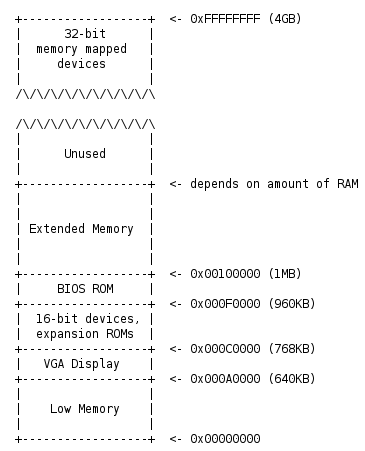
\includegraphics{memoria.png}
\caption{Esta figura mostra como os pinos de memória de um processador intel de
32 bits é ligado. Ela foi retirada de
http://pdos.csail.mit.edu/6.828/2008/labs/lab1/lab1.html}
\label{fig:memoria}
\end{center}
\end{figure}

De modo a simplificar o trabalho do desenvolvedor de kernel o grub criou a
especificação Multiboot, é um protocolo para fazer tudo que eu mencionei no
parágrafo anterior. Para o multiboot funcionar eu preciso colocar algumas
informações no meu binário, como um número que identifica que o kernel suporta
multiboot, flags para o grub saber o que carregar na memória e um checksum.

Quando eu entro na função \emph{inicio} (papagaio.s) já estou em modo protegido
e o registrador ebx aponta para a \emph{struct} com as informações que o grub
transmite para o meu kernel (include/multiboot.h).

Uma inicialização que o grub não faz é colocar o kernel no \emph{higher half} do
endereço virtual. Isso se faz necessário porque um pedaço do endereçamento
virtual dos processos será sempre o kernel. Ainda não está muito claro para mim por
que isso é necessário, mas pelo que me foi dito tem alguma relação com o
funcionamento do TSS e também parece que o desempenho é melhor dessa forma no
x86. Parece reduzir a quantidade de mudanças necessárias numa troca de contexto.

O \emph{linux}, pelo que eu li, parece se carregar a partir do endereço
0xC0000000 da memória virtual. Ou seja, um processo nunca poderá acessar
endereços a partir de 0xC0000000 O endereço virtual é aquele que é traduzido,
através da paginação, em um endereço real. O capítulo seguinte entrará em mais
detalhes sobre o funcionamento da paginação.

Eu explorei algumas formas para fazer isso (colocar o kernel na \emph{higher
half}). O que eu gostaria era apenas dar um \emph{push ebx} e \emph{call kmain}
dentro de papagaio.s. Entretanto, se eu linkar o kernel todo como se
ele estivesse na \emph{higher half} do endereço virtual, qualquer simbolo da
memória que eu acesse será invalido até que o hardware faça a tradução correta
do endereço. Assim, a idéia é fazer essa tradução de forma temporária no inicio,
pular para o código C e, então, carregar a forma definitiva de
mapeamento~\footnote{O que eu acabei escolhendo foi o esquema na
seção~\ref{subsec:paginacao_4MB}.  Mas outras possibilidades consideradas estão
aí também para os interessadosa.}.

\subsection{O truque de Tim Robinson}
Pesquisando a Internet a primeira forma que eu descobri de fazer essa passagem
foi o truque de Tim Robinson (Tim Robinson's trick).

Quem é Tim Robinson? De onde surgiu? Quando ele fez esse truque? Para que
sistema operacional? Quais eram os motivos dele? São todas perguntas que eu não
tenho resposta. Dentre tantas perguntas que eu nunca respondi, essas parecem ser
as mais simples delas no momento.

O truque usa segmentação. Um segmento tem um endereço base e um limite. O
endereço virtual é somado com a base, originando o endereço linear (que deve ser
menor que o limite). O truque consiste em usar essa soma para, na verdade, fazer
uma subtração no valor de memória.

No exemplo que eu
encontrei~\footnote{http://wiki.osdev.org/Higher\_Half\_With\_GDT} o kernel era
linkado em 0xC0000000 e o valor a ser somado é 0x40000000. Se você não entende
porque 0xC0000000 + 0x40000000 = 0, então sugiro que você estude sobre
complemento de dois. Verá que 0x40000000 = -0xC0000000.

Uma vez que você entende o funcionamento dos segmentos, esse método é realmente
muito simples. O código~\ref{codigo:timrobinson_trick} mostra o que é necssário
para fazer o truque. É uma forma muito simples de atingir nosso objetivo.

\begin{codigo}
\begin{verbatim}
inicio:
        ; As instruções seguintes carregam os registradores de
        ; segmento depois de carregar o nosso GDT.
        lgdt [truque]
        mov ax, 0x10
        mov ds, ax
        mov es, ax
        mov fs, ax
        mov gs, ax
        mov ss, ax

        ; Para fazer o registrador cs utilizar o gdt que
        ; carregamos nós precisamos fazer um jmp.
        jmp 0x08:higherhalf
higherhalf:
        add ebx, 0xc0000000
        push ebx
        call kmain
[section .comeco]
;
; O header para comunicação multiboot deve ficar aqui.
;
truque:
        dw fim_gdt - gdt - 1 ; tamanho do GDT
        dd gdt ; endereço linear do GDT
gdt:
        dd 0, 0 ; null gate
        ; code selector 0x08: base 0x40000000, limite 0xFFFFFFFF,
        ; tipo 0x9A, granularidade 0xCF
        db 0xFF, 0xFF, 0, 0, 0, 10011010b, 11001111b, 0x40
        ; data selector 0x10: base 0x40000000, limite 0xFFFFFFFF,
        ; tipo 0x92, granularidade 0xCF
        db 0xFF, 0xFF, 0, 0, 0, 10010010b, 11001111b, 0x40
fim_gdt:
\end{verbatim}
\caption{Este código foi adaptado de
http://wiki.osdev.org/Higher\_Half\_With\_GDT. A seção \emph{.comeco} deve ser
linkada em 0x100000 mesmo. O resto do kernel fica em 0xC0000000.}
\label{codigo:timrobinson_trick}
\end{codigo}

Nesse código já podemos ver o primeiro problema com o método. O grub coloca no
registrador \emph{ebx} o valor do endereço físico em que se encontra a tabela de
informações do multiboot. Assim, se quisermos acessar o endereço após o truque é
necessário somar 0xC0000000, afinal, o truque efetivamente subtrai 0xC0000000 de
qualquer endereço. A tabela do multiboot é uma coleção de endereços, então
precisaremos fazer essa soma em todos os endereços. Se quisermos poder imprimir
algo na tela, iremos precisar acessar ao endereço 0xB8000, que também
precisaria ser somado.

Eu preciso das informações da tabela do multiboot para criar inicializar, de
forma definitiva, o sistema de controle de endereços virtuais e gostaria
de utilizar minha função de imprimir para debugar o meu código. Assim, o truque
acaba tornando as coisas mais chatas, durante parte do funcionamento do kernel
eu precisaria somar 0xC0000000 aos endereços físicos.

\subsection{Truque da paginação com 4KB}
O que eu realmente preciso é poder tratar tanto os endereços virtuais quanto os
físicos da mesma forma. O esquema de paginação pode me ajudar a solucionar esse
problema.

Montei uma \emph{page table} e \emph{directory table} utilizando assembly
de forma que todos endereços da máquina apontassem para os primeiros 4MB de RAM.
Para fazer isso eu utilizei o código~\ref{codigo:pagina_trick}. Note que todas
entradas no diretório apontam para a mesma tabela de páginas que faz um
mapeamento 1:1. Ou seja, se o número da página no endereço virtual é 1, a tabela
de página também mapeia para 1.

\begin{codigo}
\begin{verbatim}
inicio:
        mov ecx, 1023
        mov [0x0], dword 0x1003
loop_diretorio:
        mov eax, ecx
        shl eax, 2
        mov [eax], dword 0x1003
        loop loop_diretorio

        mov ecx, 1023
        mov [0x1000], dword 0x13
loop_tabela:
        mov eax, ecx
        mov edx, ecx
        shl eax, 2
        shl edx, 12
        add eax, 0x1000
        or edx, 0x13
        mov [eax], edx
        loop loop_tabela

        mov eax, 0x0
        mov cr3, eax
        mov edx, cr0
        or edx, 0x80000000
        mov cr0, edx
\end{verbatim}
\caption{Cria um diretório e uma tabela de páginas no começo da
memória (nas duas primeiras páginas de memória).}
\label{codigo:pagina_trick}
\end{codigo}

Em outras palavras, configurando a tabela de páginas dessa forma nós ignoramos
os primeiros 10 bits dos endereços e mapeamos os restantes 22 bits no primeiro
MB de memória física.

Como o kernel começa em 0xC0100000, se retiramos os 10 primeiros bits, temos
0x100000, o endereço real do kernel. Enquanto as estruturas do kernel que
precisamos acessar estiverem dentro do limite de 4MB, tudo funcionará
perfeitamente. No caso de um kernel maior, pode ser necessário dividir o
diretório em dois e mapear um espaço maior do endereço físico.

O endereço físico que o multiboot retorna também está nesse limite de 4MB
iniciais, bem como o endereço da VGA, que é 0xb8000.

\subsection{Truque da paginação 4MB}
\label{subsec:paginacao_4MB}
Esta é a abordagem que eu decidi utilizar. Ela é, na verdade, a mesma coisa da
abordagem anterior, mas utilizando páginas de 4MB ao invés de 4KB. Quando usamos
páginas de 4MB o processador usa apenas um nível de tabela de páginas. Assim, só
precisamos preencher o diretório de forma que todas entradas apontem para a
primeira página da memória. Dessa forma obtemos o mesmo efeito da seção
anterior, mas escreveremos menos código. O código~\ref{codigo:pagina4MB_trick}
mostra como fazer isso.

\begin{codigo}
\begin{verbatim}
inicio:
        mov ecx, 0
preenche_tabela:
        mov eax, ecx
        shl eax, 2
        mov [eax], dword 0x19b
        cmp ecx, 1024
        inc ecx
        jb preenche_tabela

        mov eax, 0
        mov cr3, eax

        mov edx, cr4
        or edx, 1<<4
        mov cr4, edx

        mov eax, cr0
        or eax, 0x80000000
        mov cr0, eax

        push ebx 

        call kmain
\end{verbatim}
\caption{Ativa paginação com páginas de 4MB e cria um diretório que aponta para
a primeira página do sistema (página 0).}
\label{codigo:pagina4MB_trick}
\end{codigo}

Esta abordagem necessita de mais código que o truque de Tim Robinson, mas
funciona melhor para minhas necessidades. Além disso, a parte mais complicada do
código necessário é um simples \emph{loop} com contador. É até interessante
fazê-lo para treinar um pouco o Assembly :-P.

\section{Gerencia de Memória}
\subsection{Revisão sobre Paginação}
Aqui reviso um pouco sobre a páginação, porque eu mesmo precisava refrescar o
assunto na minha cabeça, mas este aqui com certeza não é um guia sobre as idéias
por trás da paginação. Se você quer aprender a respeito sugiro ``Operating
System Concepts'' do Silberschatz (existe tradução do livro para o português).
Nele existem vários outros conceitos importantes para sistemas operacionais.

Gerenciar a memória em páginas é teoricamente bastante simples. Primeiro
dividimos todo espaço enderessável (4GB na arquitetura 32 bits) em páginas de
4KB cada. Cada uma dessas páginas podem estar no disco, podem estar na memória
principal ou podem nem mesmo existir. A figura~\ref{pagina}, retirada do manual
da Intel, mostra bem o funcionamento do mecanismo.

\begin{figure}
	\begin{center}
	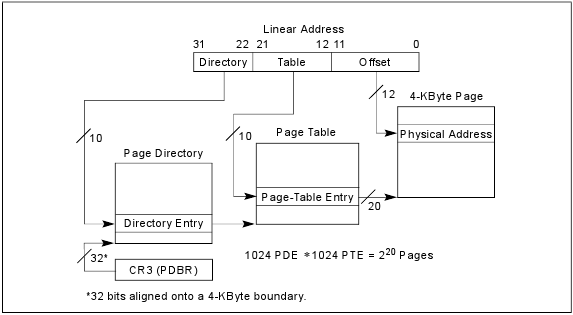
\includegraphics[scale=0.8]{paginacao}
	\end{center}
	\caption{Funcionamento da paginação na arquitetura x86.}
	\label{pagina}
\end{figure}

Se dividirmos um espaço de 4GB em pedaços de 4KB, nós temos $2^{20}$ pedaços.
Vamos fazer as contas mais precisamente para termos certeza:
\begin{eqnarray*}
	4 GB & = & 4,194,304 KB \\
	2^{20} & = & 1,048,576 \\
	\frac{4,194,304}{4} & = & 1,048,576
\end{eqnarray*}
Dessa forma fica claro porque existem 20 bits reservados para o diretorio de
páginas (page-directory) e tabela de páginas (page-table). Esse é o número total
de páginas.

Numa arquitetura mais simples poderiamos ter só uma grande tabela de páginas
endereçada usando esses 20 bits, essa tabela seria responsável para transformar
esse endereço linear\footnote{Na nomenclatura da Intel um endereço virtual é o
endereço antes de segmentação e endereço linear é o endereço após a segmentação
mas antes da transformação pelas páginas. Como a segmentação será
desconsiderada, poderiamos chamar o endereço linear de virtual.} em um endereço
real. Isso é, no seu endereço linear você aponta para uma das páginas na tabela
de páginas, essa página ganha um endereço novo, o endereço na memória RAM do
hardware. Note que os bytes dentro de uma página são acessados através do
offset. Dentro de uma página de 4KB para acessar byte a byte precisamos de 12
bits -- basta fazer as contas para conferir.

A Intel preferiu fazer uma arquitetura com duas indireções: um diretório de
páginas e uma tabela de páginas. Tanto o diretório quanto cada uma das tabelas
de página cabem em \emph{exatamente} uma página. No futuro isso nos irá ajudar
porque nem essas páginas precisam estar o tempo todo na memória.

\subsection{Implementação}

\end{document}
